\newpage
\setcounter{section}{8}
\sectionmark{Προδ. μεθόδου υλοποίησης \& χρονοπρογραμματισμός}
\setcounter{section}{7}
\section[Προδιαγραφή μεθόδου υλοποίησης και χρονοπρογραμματισμός]{Προδιαγραφή μεθόδου υλοποίησης \\και χρονοπρογραμματισμός}
\sectionmark{Προδ. μεθόδου υλοποίησης \& χρονοπρογραμματισμός} 
\label{section:3-8-implementation-methodology-specification}

Κατά τον χρονοπρογραμματισμό υιοθετήθηκαν οι τακτικές που ορίζει το Scrum. Το συνολικό προγραμματιστικό έργο χωρίστηκε σε επιμέρους διακριτούς στόχους και κάθε στόχος αντιστοιχήθηκε σε ένα Sprint. Η εργασία κάθε Sprint διαχωρίστηκε περαιτέρω σε επιμέρους epic. Ωστόσο, σε αυτό το στάδιο χρονοπρογραμματισμού δεν έγινε αναλυτικότερη περιγραφή των task των epic, διαδικασία που πραγματοποιήθηκε κατά το αρχικό στάδιο της υλοποίησης των τελευταίων.

Ως σημαντικότερος στόχος της ανάπτυξης ορίζεται η δημιουργία ενός ελάχιστου βιώσιμου προϊόντος (Minumum Viable Product - MVP). Σε αυτόν τον στόχο περιλαμβάνονται οι πιο στοιχειώδεις λειτουργίες μίας πλατφόρμας επικοινωνίας οι οποίες την κάνουν χρήσιμη, δηλαδή η δυνατότητα εγγραφής, δημιουργίας θεμάτων και μηνυμάτων και ανάγνωσης του υπάρχοντος περιεχομένου. Επειδή ο στόχος αυτός περιέχει από μόνος του σημαντική πολυπλοκότητα και δυσκολία κρίθηκε αναγκαίος ο περαιτέρω διαχωρισμός του σε τρία Sprint.

Στο πρώτο Sprint ορίστηκε ο στόχος της δημιουργίας μίας βάσης κώδικα (codebase), της εξοικείωσης με τα προγραμματιστικά εργαλεία του οικοσυστήματος των DApp και της επιτυχούς δημιουργίας του πρώτου έξυπνου συμβολαίου. Ως στόχος του δεύτερου Sprint ορίστηκε η δημιουργία των τεχνικών χαρακτηριστικών που αφορούν στους χρήστες της εφαρμογής και που οι ίδιοι έχουν συνηθίσει να αναμένουν από μία τέτοια πλατφόρμα. Στο τρίτο Sprint συμπεριλήφθηκαν τα τεχνικά χαρακτηριστικά που απομένουν ώστε να δημιουργηθεί το MVP.

Τα επόμενα τρία Sprint χτίζουν διαδοχικά πάνω στην υπάρχουσα δουλειά και υποδομή. Στο τέταρτο μέρος εργασίας ορίστηκε ως στόχος η προσθήκη των δυνατοτήτων της ψηφοφορίας επί των μηνυμάτων, καθώς και της δημιουργίας ψηφοφοριών (polls) στα θέματα. Το επόμενο Sprint περιλαμβάνει εργασίες δημιουργίας υποδομής και την πρώτη ημι-δημόσια εγκατάσταση της εφαρμογής σε περιβάλλον δοκιμής. Το τελευταίο Sprint αποτελεί το τελικό προϊόν και περιέχει task σχετικά με τη δημιουργία κοινοτήτων και τη beta εγκατάσταση της εφαρμογής.

\newpage
Εποπτικά, η διαδικασία της υλοποίησης περιγράφεται στο παρακάτω σχήμα:

\vspace{\baselineskip}

\begin{figure}[H]
    \centering
    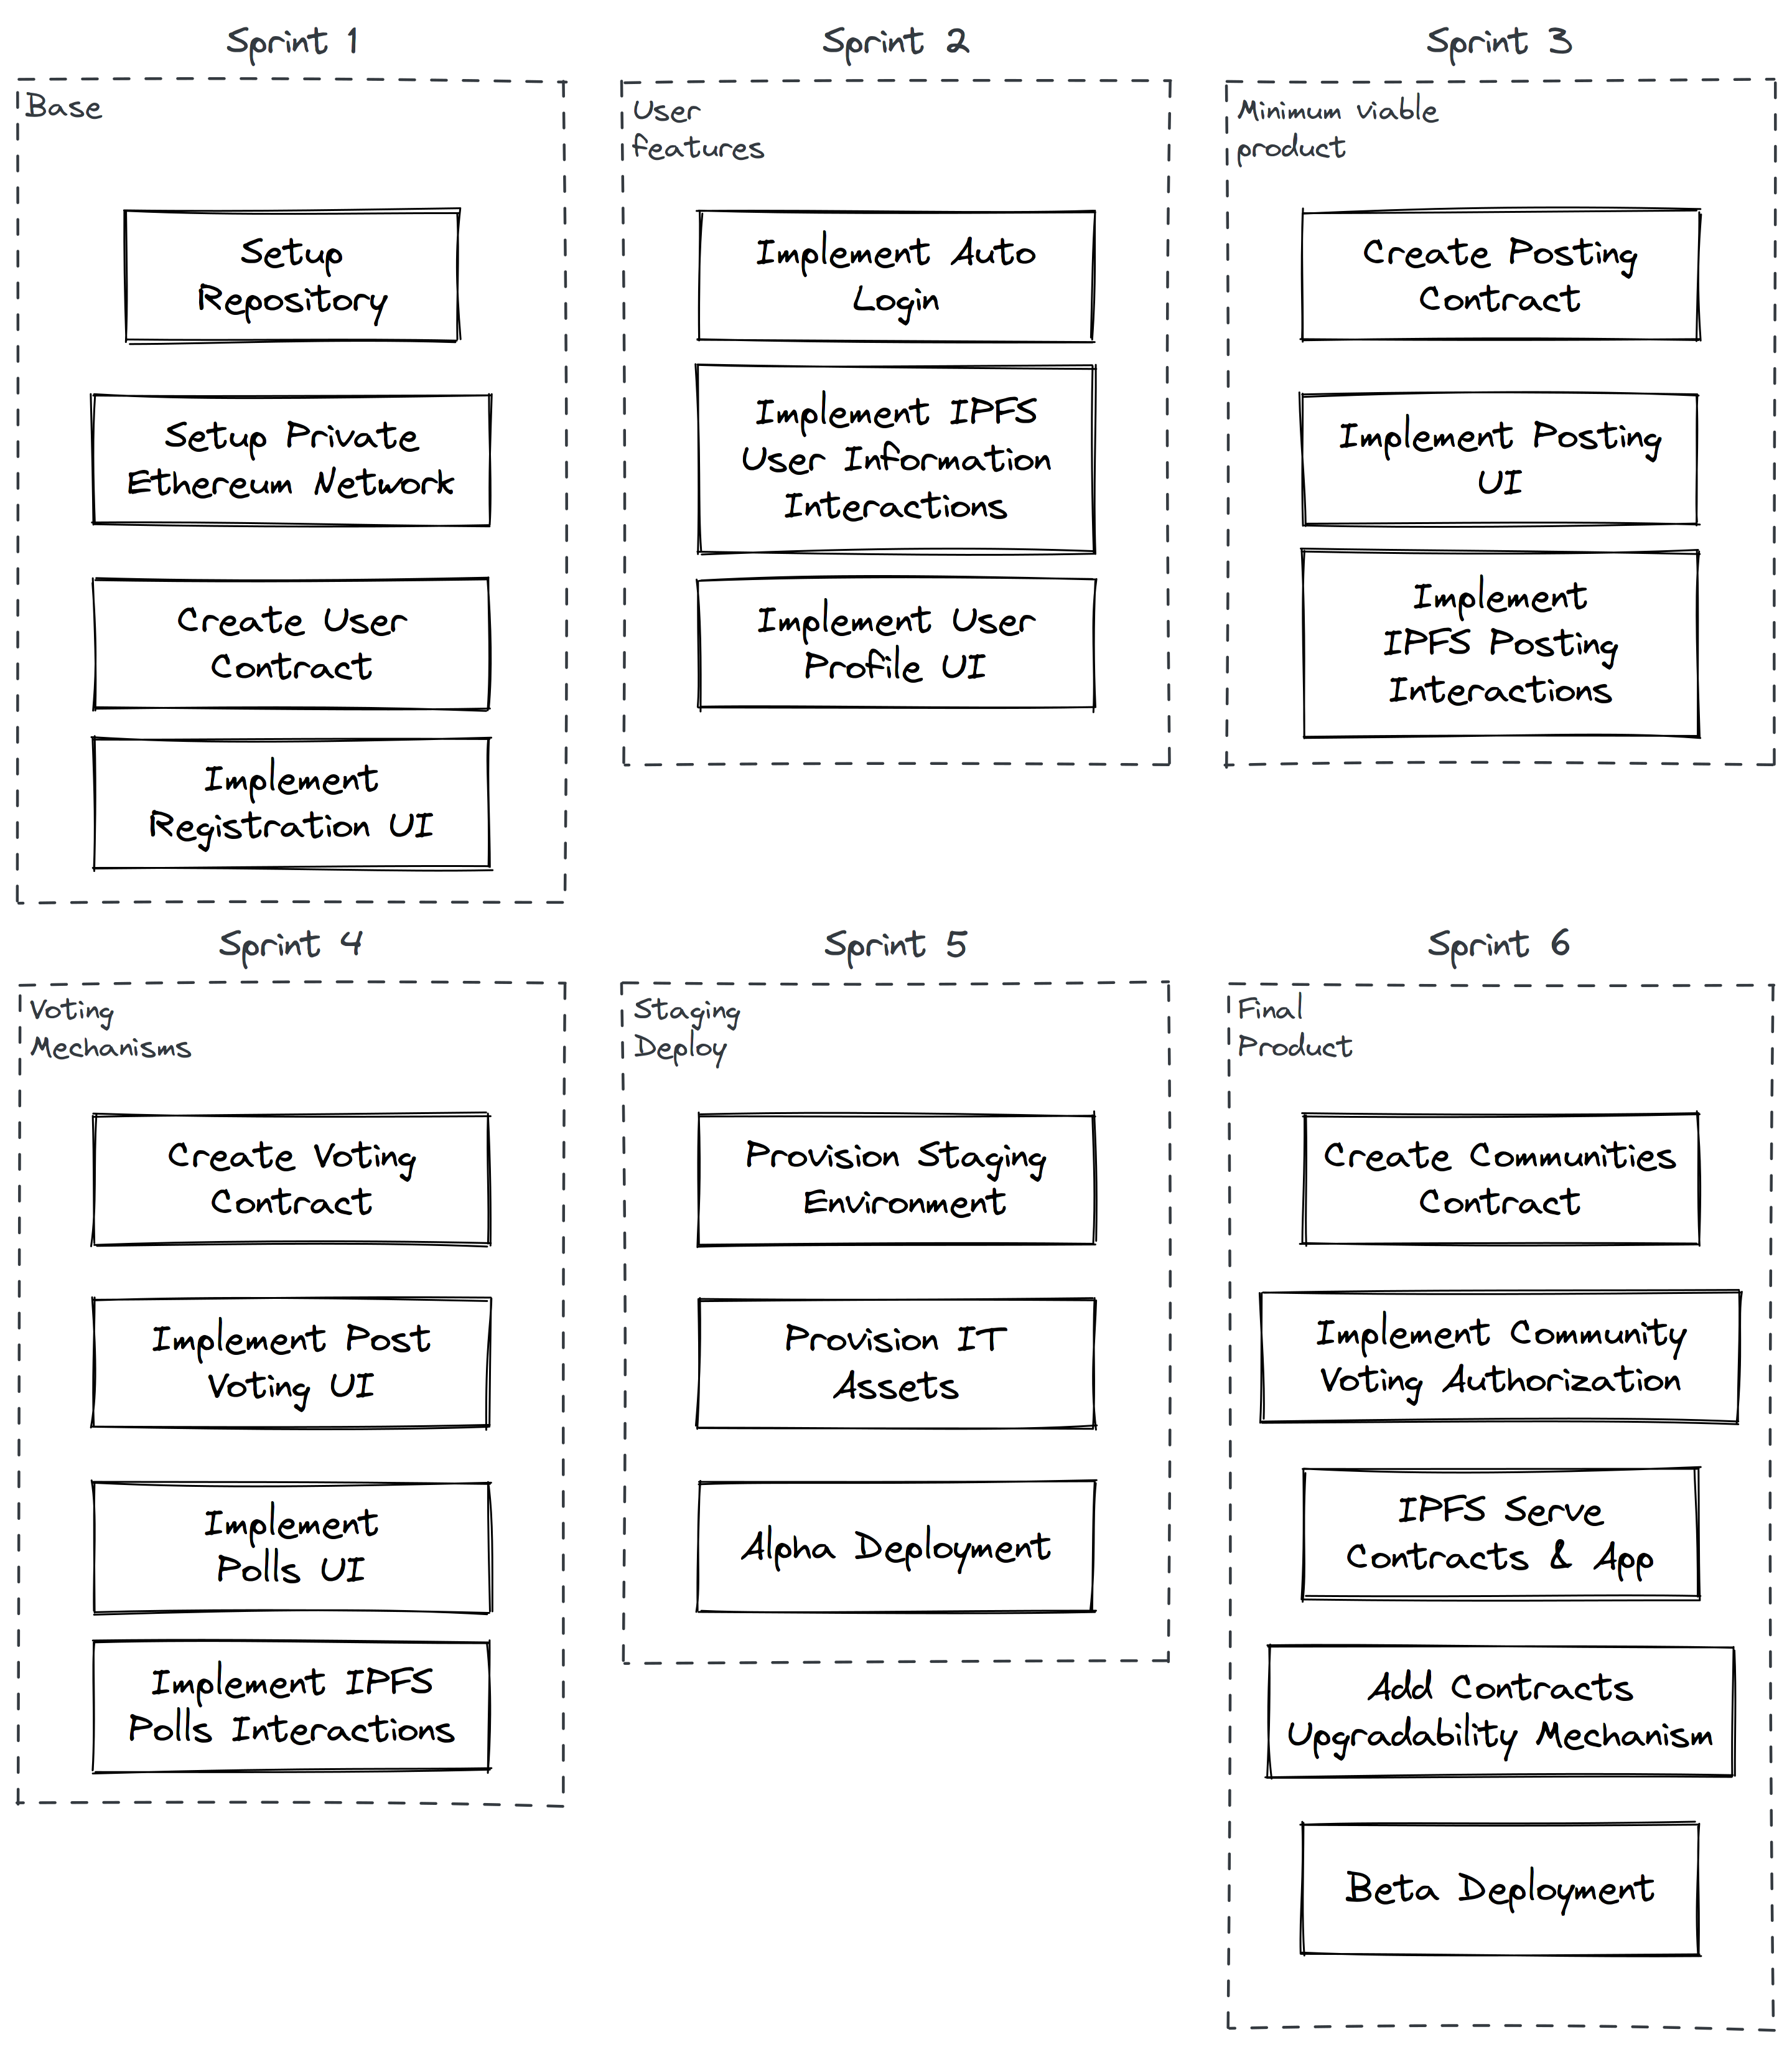
\includegraphics[width=\textwidth]{assets/figures/chapter-3/3.8.implementation-methodology-specification-sprints.png}
    \caption{Διαχωρισμός σε Sprint (στάδιο σχεδίασης)}
    \label{figure:3.8.implementation-methodology-specification-sprints}
\end{figure}
